\chapter{Image Manipulation}
\vspace{-10mm}

Dicom-Presenter is an application for viewing image data. Entire image manipulation was solved with use of OpenGL\citesec{openglhome} library in an early version of Dicom-Presenter. OpenGL was used for image storing, for changing image properties and for drawing images on screen. Unfortunately, OpenGL brought complications to application compatibility with various types of hardware. Therefore, the author of this work decided to remove OpenGL from application and replace all classes using OpenGL with their non-OpenGL equivalents. 

Before rewriting all image processing classes without OpenGL, there was a need to study how to complete all image processing tasks without OpenGL. Moreover, OpenGL uses GPU to perform its tasks, so there was a need to calculate the loss of performance if OpenGL would be removed. 

\section{Image Storing}
\label{rawdata}
There are two different libraries used for image manipulation in Dicom-Presenter. DCMTK library\citesec{dcmtkhome} is used for loading images from hard disk, while Qt library (formerly OpenGL) is used for displaying images on computer screen. DCMTK library must be used since it supports loading files in DICOM format, moreover some application framework must be used for image displaying. It offers loading compressed image files and saving them uncompressed into RAM memory. To be able to display this raw data properly by Qt library, it is necessary to understand the way image data is represented in a computer. 

A color image consisting of $m \cdot n$ points (pixels) can be described by $m \cdot n$ number triads. The triads would be coordinates in RGB or HSV color space\footnote{Colors which can be displayed can be fully described by three values. This fact is based on human eye anatomy and leads to construction of coordinate systems describing each displayable color. Coordinates of RGB color space are red, blue, green color while hue, saturation, value are coordinates in HSV color space.} \cite[page~211]{imageprocessingintroduction}. Data in a computer is stored in elementary units - bytes, which can hold 256 different values. Each byte consists of eight unitary units - bits ($2^8 = 256 $). If considered that one byte can include color information of only one pixel, then only eight-bit multiples can be used for pixel color storage: 8 bits, 16 bits, 24 bits, etc.\cite[page~208]{colorphotography} In case of 24 bit color depth, three bytes are used for pixel color storage - each byte for each color. If 8 bits depth or 16 bits depth is used, in both cases the bit numbers are not divisible by three, so there are several ways that bits among colors can be distributed.
 
Qt library uses three different formats of 16 bit color information storage\cite{QtDoc}. The formats differ by number of bits distributed to each color and are described by triads of numbers: 5-6-5, 5-5-5, 4-4-4. The first format uses 5 bits for red color, 6 bits for green color and 5 bits for blue color. The numbers of bits for each color are uneven but no redundant bits are present. Both 5-5-5 and 4-4-4 formats include redundant bits for each image pixel\cite[page~37]{fileformatencyclo}.

Qt library allows the display of images, which are actually saved in the computer memory as an array of bytes, in some of the supported formats (such as described above). Next to the color depth formats, image storage can differ by the number of bytes used for storing each image line. If an image has $m \cdot n$ pixels and two bytes are used per pixel (for example 16 bit 5-5-5), there is no rule that $m \cdot n \cdot 2$ bytes will be used. A computer memory in x86 architecture reads its data in elements called words usually consisting of 4 bytes for x86 architecture and 8 bytes for 64-bit architecture. Therefore, image data are in a computer memory are often aligned in order that that each image line starts at a beginning of some 4-byte or 8-byte word\cite{memoryalignment}. For instance, if we consider an image of $100 \cdot 100$ pixels saved with 8 bit pixel depth on 64-bit architecture, each line consisting of $100$ pixels would be saved on $128$ or bytes.

To conclude, if a picture is reconstructed from uncompressed raw data saved in computer memory, essential indications are: which color storage format is used for each pixel and which bit alignment is used for each pixel-line. These two items of information are enough for correct image reconstruction.

\subsection{Image Construction from Raw Data in Qt Library}
As mentioned in previous text, DCMTK library allows loading compressed files from hard disk and saves them into the computer memory in one of mentioned data alignment. Qt library allows the display of image data onto computer screen. It is mandatory to coordinate an output of DCMTK and an input of Qt library to be able to display an image properly.

DCMTK library offers a function which saves a copy of loaded image data into a new place in image memory in required data alignment \cite{dcmtksupport}. The function declaration is:

\clist{const void* DicomImage::getOutputData	(const int bits = 0,
const unsigned long frame = 0,
const int planar = 0 )}

The first parameter denotes a required data alignment of each pixel; the other two parameters describe the orientation of the image slice inside the three-dimensional texture. The function returns a pointer to the part of memory where image data will be stored.

Furthermore, Qt library offers a construction of its object depending on image data already stored in the computer memory. The object receives a pointer to image data through its constructor. If the image data meets prospective requirements, the object can be called to draw the image at any time, as long as the data is still retained in the computer memory.

The constructor declaration is:

\clist{QImage::QImage(uchar* data, int width, int height, int bytesPerLine, Format format)}

The first parameter is a pointer to image data already saved in computer memory. The data is declared as \clist{unsigned char} which is a C++ equivalent of a \clist{byte} type. The last parameter \clist{format} describes a pixel alignment. It describes a number of bytes used for each pixel and a particular way of color information storage. The \clist{bytesPerLine} parameter describes an image line alignment of pixel data.

Qt library itself cannot determine the exact values of above described parameters. Therefore, the parameter values must be known before. A misleading value of parameter describing pixel color storage will lead to false color interpretation of the image. Furthermore, incorrect parameter describing image line alignment can avert image loading or can cause a program failure due to unauthorized memory access\cite{QtDoc}.  


\begin{figure}
	\begin{center}
	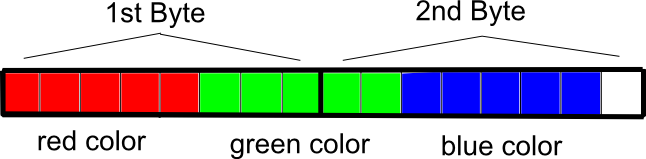
\includegraphics[width=130mm]{Text/IMG/ImageStoring_16bit.png}
	\end{center}
	\caption{A distribution of 16 bits of 2 bytes among three colors of a pixel.}
	\label{imagestoring}
\end{figure}

\section{Image Enhancement Operations}
\label{brightnesscontrast}

One of important tasks to re-implement in Dicom-Presenter was an ability to adjust image brightness and contrast. Images which will be opened in Dicom-Presenter can be captured on various MRI units with differing imaging properties. The ability to increase image brightness and contrast is mandatory in order to ensure sufficient display quality. Images that are too dark or too gray need to be brightened or need to increase contrast to ensure better observation of physiological findings. Brightness and contrast change is among DICOM users called ``windowing''.

For further needs of this text brightness and contrast need to be defined. 

A gray-scale image can be considered as a matrix of numbers\cite[p.~1]{imageprocessing}: 

\[
 Im_{res_{x},res_{y}} =
 \begin{pmatrix}
  Im(1,1) & Im(1,2) & \cdots & Im(1,res_{x}) \\
  Im(2,1) & Im(2,2) & \cdots & Im(2,res_{x}) \\
  \vdots  & \vdots  & \ddots & \vdots  \\
  Im(res_{y},1) & Im(res_{y},2) & \cdots & Im(res_{y},res_{x})
 \end{pmatrix}
\]

where $ res_{x} $, $res_{y}$ are dimensions of the image. $Im(x,y)$ is a lightness of a pixel.

Brightness then can be defined as:
\[
  Brightness(Im) = \frac{1}{res_{x}  \cdot res_{y}}\sum_{\substack{0 \leq x \leq res_{x} \\ 0 \leq y \leq res_{y}}} Im(x,y)
\]

Contrast is understood as overall difference in luminosity between bright and dark pixels. There are more possible definitions of contrast. One possible definition is\cite{contrastinimages}:

\[
Contrast(Im) = \sqrt{\frac{1}{res_{x} \cdot res_{y}}\sum_{\substack{ 0 \leq x \leq res_{x} \\ 0 \leq y \leq res_{y} }}(Im_{x,y}-Brightness(Im))^2}
\]

An argument for using these two definitions for brightness and contrast is that they are analogies for mean value and variance of set of values.

If there is a need to increase or decrease image brightness in computer applications simply a constant is added to all image points:

\begin{equation}
\label{brightness}
  Im(x,y) \longmapsto Im(x,y) + c_{brightness} 
\end{equation}

Image contrast is usually adjusted by a linear transformation applied to all image points:

\begin{equation}
\label{contrast}
  Im(x,y) \longmapsto   (Im(x,y) - 0.5) \cdot c_{contrast} + 0.5
\end{equation}

A disadvantage of both ways is that some image information is lost. Let's consider an image described by a matrix with elements of integers in range from zero to 255. Let the brightness of the picture increased according to formula \eqref{brightness} with a positive constant $ c_{brightness} $. Then all the points brighter than $ 255 - c_{brightness} $ on original image will have luminosity of 255 regardless their original luminosity. Similarly if contrast would be increased according to formula \eqref{contrast} with a constant $ c_{contrast} $ then all points brighter than $ \frac{1}{2} \cdot 255 \cdot (\frac{1}{c_{contrast}}+1) $ will have the same color (maximum white). As well all pixels darker than $ \frac{1}{2} \cdot 255 \cdot (1 - \frac{1}{c_{contrast}}) $ will have the same color (maximum black).

\subsection{Non-linear contrast change}
To avoid the loss of information during a contrast change, it is possible to use a more sofisticated function. 
The function ($y=f(x,c)$) where $c$ is a parameter should meet the following conditions:
\begin{itemize}
\item $\|f(x,c) - (k \cdot x + c)\|$ should be minimal for every c
\item $y$ values for $x<\frac{1}{2} \cdot 255 \cdot (1 - \frac{1}{c_{contrast}})$ should be linearly distrubuted on negative neighborhood of $1$
\item $y$ values for $x>\frac{1}{2} \cdot 255 \cdot (\frac{1}{c_{contrast}}+1)$ should be linearly distrubuted on positive neighborhood of $0$
\end{itemize}

A function meeting the criteria was found in work \cite[page~18]{flaska_vu}. The idea was based on behavior of function $tanh(x)$ on $[-\infty,+\infty]$. The function was transformed to interval $[-\frac{1}{2},+\frac{1}{2}]$; shifted to point $x=\frac{1}{2}, y=\frac{1}{2}$ and further transformed to:

 \[ f(x,c)= \bigg[ 1-\tanh(c) \bigg] \cdot \left(1-\frac{1}{2}\right) + \frac{1}{2} \cdot \tanh\left[ 2 \cdot c \cdot \left(x - \frac{1}{2}\right) \right] + \frac{1}{2} \]

\subsection{Pixel Manipulations in Qt}

Qt library doesn't offer its own functions for elementary pixel manipulations such as change of brightness and contrast. These operations (described in Section \ref{brightnesscontrast}) must be done in application source code for each image pixel.

A change of brightness or contrast of an image of $m \cdot n$ pixels will be undertaken in $m \cdot n$ steps. In each step a color of the pixel must be obtained, new color value will be calculated and the value will be saved into the picture. Qt library offers two ways to perform the task: pixel manipulation functions or direct memory access.

If pre-implemented Qt pixel manipulation functions are used, the source code will be following:
\begin{comment}
\begin{lstlisting}[label=qtcontrast,caption={Image enhancement operations implementation using Qt library functions for pixel manipulation.},escapeinside={@}{@}]
QImage image(...);
for (int y=0; y<height; y++) {
	for (int x=0; x<width; x++) {
		@\label{lst:pixel}@QRgb color = image.pixel(x,y);
		@\label{lst:operation}@QRgb newcolor = qRgb(func1(qRed(color)),func2(qGreen(color)),func3(qBlue(color)));
		@\label{lst:setPixel}@image.setPixel(x,y,color);
	}
}
\end{lstlisting}
\end{comment}
Function \clist{QRgb QImage::pixel(int x,int y)} is used to retrieve color information of a pixel. Function \clist{void QImage::setPixel(int x,int y,QRgb rgb)} is used to save the color information back to the picture. Due to multi-thread programming support the \clist{QImage::setPixel} function offers low performance. Within each function call Qt library must attach and detach a process to shared memory segment where the image data are stored. These steps are performance expensive.

Nevertheless, Qt library offers a high performance option to change image pixel data. Image data are modified directly inside the computer memory without a function call from QImage class. A function from QImage class is called just to retrieve a pointer to memory segment containing image data. The code will be following:

\begin{lstlisting}[label=fastcontrast,caption={Image enhancement operations performed by direct access into computer memory.},escapeinside={@}{@}]
QImage image(...);
for (int y=0; y<height; y++) {
	@\label{lst:pixel-fast}@QRgb* imageLine=(QRgb*)image.scanLine(y);
	@\label{lst:for}@for (int x=0; x<width; x++) {
		@\label{lst:qrgb}@imageLine[x] = qRgb(func1(qRed(imageLine[x])),func2(qGreen(imageLine[x])),func3(qBlue(imageLine[x])));
	}
}
\end{lstlisting}

Function \clist{QImage::scanLine(int y)} returns a pointer to a segment of memory where is saved \clist{y}-th line of the image. The \clist{QImage::scanLine(int y)} function returns a pointer to \clist{unsigned char} array (byte array). The conversion to \clist{QRgb} array together with using Qt functions for changing pixel data (line \ref{lst:qrgb}) will remove necessary byte conversions related to pixel data alignment. If working with the \clist{unsigned char} array, data alignment rules must be respected. The for-cycle browsing through each image line (line \ref{lst:for}) would be ranged to \clist{2*width}, which is actually the real size of an image line in computer memory (expressed in bytes at 16-bit color depth).


\section{Image Rendering}
\label{rendering}
Qt library offers several ways how to create and render graphic scene composing of existing images stored on hard disk. The library includes three different classes which can hold bitmap data: QImage, QPixmap, QPicture. All the classes can act as a scene to be painted onto as well as can be a pattern to be painted. Differences among these classes are\cite{QtDoc}:

\begin{itemize}
\item QImage class is optimized for reading and writing images from/into a hard disk and for direct pixel access and manipulation.
\item QPixmap class is optimized for on-screen rendering.
\item QPicture class can record a history of received painting requests and replay them.
\end{itemize}

Therefore, among other possible ways, the most reasonable solution for rendering existing images from hard

\begin{enumerate}
  \item Save and hold image data in computer memory with QImage objects.
  \item Perform image enhancement operations inside QImage objects.
  \item Paint the content of QImage objects into a QPixmap object to assemble user's workspace.
  \item Paint the QPixmap object to the computer screen.
\end{enumerate}

To paint any object of the mentioned classes inside another object of the classes, Qt library offers a QPainter class. A process of drawing an existing image into a QPixmap scene can be found on Listing \ref{painting}.

\begin{lstlisting}[label=painting,caption={A process of assembling user's desktop from existing images and rendering it to computer screen.},escapeinside={@}{@}]
@\label{lst:qimage}@QImage* image = new QImage(data,width, height,align);
@\label{lst:qpixmap}@QPixmap* pixmap = new QPixmap(Width, Height);
@\label{lst:qpainter}@QPainter* painter = new QPainter();
@\label{lst:begin}@painter->begin((QPaintDevice*)pixmap);
QRect position(QPoint(x,y),QPoint(w,h));
@\label{lst:draw}@painter->drawImage(position,image);
painter->end();
QLabel *label = new QLabel();
@\label{lst:render1}@label->setPixmap(*pixmap);
@\label{lst:render2}@label->update();
\end{lstlisting}

There is a \clist{QImage} object construction on line \ref{lst:qimage}. QImage object is created to provide manipulation with image data already stored in computer memory at location referenced by pointer \clist{data}. Image data will be printed to some position into a \clist{QPixmap} object which is created on line \ref{lst:qpixmap}. This step is needed to perform the assembly of user's workspace from various visual elements. A \clist{QPainter} object created on line \ref{lst:qpainter} allows the printing of a \clist{QImage} object into a \clist{QPixmap} object. A target scene where to \clist{QPainter} object will render must be declared by \clist{::begin()} command (line \ref{lst:begin}). The existing image is printed on declared position on line \ref{lst:draw}. Finally, the workspace is rendered to user's screen on lines \ref{lst:render1} and \ref{lst:render1}.


\section{OpenGL and Qt performance}
Before the OpenGL library could be removed from the application, the impact to the application performance must be estimated. Dicom-Presenter attained 90 frames per second while performing image manipulations such as zoom, contrast change, etc. If the performance after removing OpenGL would be estimated over 30 FPS, OpenGL could be removed. 

When Dicom-Presenter is running, the aplication must perform rendering and other necessary actions each moment. The absence of OpenGL will affect only the rendering part. Therefore, simple model applications were created - these applications performed image manipulations used in Dicom-Presenter. Each task was implemented in OpenGL and without OpenGL and the applications had no other responsibilities. These applications give answer to the question of how much will be rendering affected itself. To estimate the overall performance of Dicom-Presenter, the following account was performed.
 
Consider that the Dicom-Presenter's performance is $f$ frames per second. Thus, the application needs $t=\frac{1}{f}$ seconds to perform all actions necesarry to display one screen image.  Some part of $t$ is consumed by rendering $t_{r}$; the rest is used to perform other actions $t_{o}$. So the complete time to prepare one screen image is a sum of both: $t=t_{r}+t_{o}$. Thus, if OpenGL rendering would be replaced by software rendering in Dicom-Presenter, then the time needed to prepare new screen image would be:
\begin{equation} \label{T}
T=t_{o} + t_{s}
\end{equation} 
The time necessary perform rendering can be estimated from the model application $t_{r} = \frac{1}{f_{r}}$. And it is also possible to estimate the time needed to do rendering without OpenGL - $t_{s} = \frac{1}{f_{s}}$.

Since both $t_{r}$ and $t_{s}$ are estimable values and $t_{o}$ is unknown, the equation \ref{T} can be modified:

\begin{equation} \label{T}
T = t - t_{r} + t_{s}
\end{equation} 

after substitution:

\begin{equation} \label{T}
T = \frac{1}{f} - \frac{1}{f_{r}} + \frac{1}{f_{s}}
\end{equation} 

Finally, the performance of Dicom-Presenter without OpenGL can be estimated as:

\begin{equation} \label{estimate}
F = \left(\frac{1}{f} - \frac{1}{f_{r}} + \frac{1}{f_{s}}\right)^{-1}
\end{equation}

There were significant differences in performance of the model applications. For example image contrast change was six times faster, when using OpenGL (See Table \ref{results}). Still, Dicom-Presenter should display more than 35 frames per second, altough OpenGL would be removed. It is satisfactory performance, so the library was removed (See Section \ref{noOpenGL}).

\begin{table}
\begin{center}
\caption{A performance, reached while performing simple image manipulation tasks only.\label{results}}
  \begin{tabular}{| l || l | l | }
	\hline
	Task & Used technology  & Frames per Second \\
    \hline \hline
    Image moving & Qt & 90 \\ \hline
    Image Mmving & OpenGL & 600 \\ \hline
    Contrast change & Qt & 50 \\ \hline
	Contrast change & OpenGL & 250 \\
    \hline
  \end{tabular}
  \end{center}
\end{table}




